\section{Der Algorithmus von van Kreveld}

Die Laufzeit des naiven Algorithmus in $O(n^3)$ liegt (wobei $n$ das Maximum aus Breite und Höhe des DEM ist), gibt es einige Überlegungen zu 
schnelleren Algorithmen. Als eine Art untere Schranke für die Laufzeit der viewshed-Berechnung kann das Einlesen des DEMs gesehen werden, welches 
in $O(n^2)$ liegt. Somit sollte eine Verbesserung der Laufzeit möglichst nahe an diese untere Schranke heranreichen. Im Paper von van Kreveld 
\cite{vanKrev} werden Optimierungsvorschläge vorgestellt und gezeigt, dass die Laufzeit auf $O(n^2)\log n$ verbessert werden kann. 

\subsection{Der sweep-Algorithmus}
Van Krevelds Algorithmus beruht auf dem Prinzip der sogenannten ``sweep line''. Allgemein ist eine sweep line eine (horizontale) Linie, 
welche über eine Menge von Objekten in einer Ebene ``streicht'' und dabei alle relevanten Informationen bezüglich einer Problemstellung ausliest und 
sammelt, damit diese dann weiterverarbeitet werden können. Beispielsweise kann die Linie über eine Ebene streichen und dabei den Beginn und das Ende 
geometrischer Formen detektieren (siehe Abbildung \ref{sweep}). Da sich die Menge der Objekte, die die Linie schneiden, oft ändert, muss für das 
Sammeln der Informationen eine flexible Datenstruktur gewählt werden. Hierfür eignet sich ein balancierter binärer Baum, welcher als ``Statusstruktur''
bezeichnet wird (siehe Abbildung \ref{stat}) und die Änderungen des Status festzuhalten. 

\begin{figure}[!ht]
\begin{minipage}{0.55\textwidth}
\centering
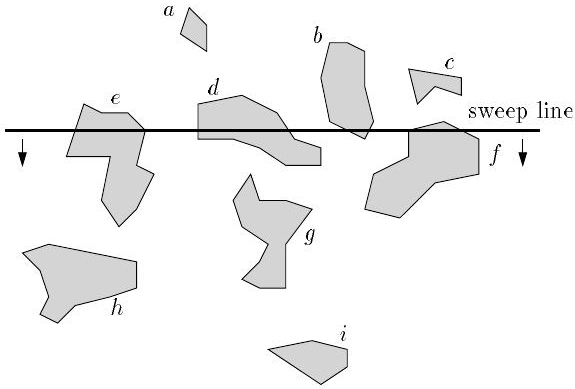
\includegraphics[scale=0.62]{bilder/sweep}
\caption{sweep line streicht über Objekte in einer Ebene}
\label{sweep}
\end{minipage}
\hfill
\begin{minipage}{0.4\textwidth}
\centering
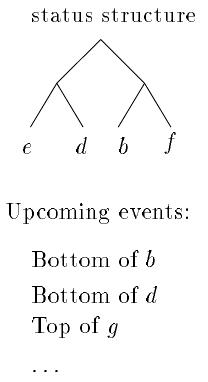
\includegraphics[scale=0.67]{bilder/statstruc}
\caption{Statusstruktur, in der die auftretenden Ereignisse gespeichert werden}
\label{stat}
\end{minipage}
\end{figure}

Um zu wissen, wann sich der Status ändert -- also wenn die Linie beispielsweise ein neues Objekt schneidet -- werden sogenannte ``events'' eingeführt
und ebenfalls in einer eigenen Datenstruktur gespeichert. Hierfür kann eine Prioritätswarteschlange oder ebenfalls ein balancierter binärer Baum 
benutzt werden. Für das Beispiel der viewshed-Analyse sind folgende events sinnvoll: 
\begin{itemize}
 \item die sweep line detektiert beim Streichen über das DEM einen neuen Pixel
 \item die sweep line detektiert beim Streichen über das DEM den Mittelpunkt eines Pixels
 \item die sweep line detektiert beim Streichen über das DEM die letzte Ecke eines Pixels, er wurde also von der Linie komplett durchlaufen
\end{itemize}
